%% For double-blind review submission, w/o CCS and ACM Reference (max submission space)
\documentclass[acmsmall,review,anonymous]{acmart}\settopmatter{printfolios=true,printccs=false,printacmref=false}
%% For double-blind review submission, w/ CCS and ACM Reference
%\documentclass[acmsmall,review,anonymous]{acmart}\settopmatter{printfolios=true}
%% For single-blind review submission, w/o CCS and ACM Reference (max submission space)
%\documentclass[acmsmall,review]{acmart}\settopmatter{printfolios=true,printccs=false,printacmref=false}
%% For single-blind review submission, w/ CCS and ACM Reference
%\documentclass[acmsmall,review]{acmart}\settopmatter{printfolios=true}
%% For final camera-ready submission, w/ required CCS and ACM Reference
%\documentclass[acmsmall]{acmart}\settopmatter{}


%% Journal information
%% Supplied to authors by publisher for camera-ready submission;
%% use defaults for review submission.
\acmJournal{PACMPL}
\acmVolume{1}
\acmNumber{CONF} % CONF = POPL or ICFP or OOPSLA
\acmArticle{1}
\acmYear{2018}
\acmMonth{1}
\acmDOI{} % \acmDOI{10.1145/nnnnnnn.nnnnnnn}
\startPage{1}

%% Copyright information
%% Supplied to authors (based on authors' rights management selection;
%% see authors.acm.org) by publisher for camera-ready submission;
%% use 'none' for review submission.
\setcopyright{none}
%\setcopyright{acmcopyright}
%\setcopyright{acmlicensed}
%\setcopyright{rightsretained}
%\copyrightyear{2018}           %% If different from \acmYear

%% Bibliography style
\bibliographystyle{ACM-Reference-Format}
%% Citation style
%% Note: author/year citations are required for papers published as an
%% issue of PACMPL.
\citestyle{acmauthoryear}   %% For author/year citations


%%%%%%%%%%%%%%%%%%%%%%%%%%%%%%%%%%%%%%%%%%%%%%%%%%%%%%%%%%%%%%%%%%%%%%
%% Note: Authors migrating a paper from PACMPL format to traditional
%% SIGPLAN proceedings format must update the '\documentclass' and
%% topmatter commands above; see 'acmart-sigplanproc-template.tex'.
%%%%%%%%%%%%%%%%%%%%%%%%%%%%%%%%%%%%%%%%%%%%%%%%%%%%%%%%%%%%%%%%%%%%%%


%% Some recommended packages.
\usepackage{proof}
\usepackage{amsmath,amssymb,amsthm,textcomp}

\usepackage{booktabs}   %% For formal tables:
                        %% http://ctan.org/pkg/booktabs
\usepackage{wrapfig}
\usepackage{subcaption} %% For complex figures with subfigures/subcaptions
                        %% http://ctan.org/pkg/subcaption

\usepackage{url}
\usepackage{xspace}

\usepackage{fancyvrb}
\fvset{fontsize=\smaller}

\usepackage{color}

\usepackage{cleveref}
\usepackage{hyperref}

% \usepackage[svgnames]{xcolor}
%   \definecolor{diffstart}{named}{Grey}
%   \definecolor{diffincl}{named}{Green}
%   \definecolor{diffrem}{named}{OrangeRed}

% \usepackage{listings}
%   \lstdefinelanguage{diff}{
%     basicstyle=\ttfamily\small,
%     morecomment=[f][\color{Dark gray}]{@@},
%     morecomment=[f][\color{Forest green}]{+\ },
%     morecomment=[f][\color{Firebrick}]{-\ },
%   }
% % \lstset{numbers=left,numberblanklines=false,escapeinside=||}
% \lstset{escapeinside=||}
% \let\origthelstnumber\thelstnumber
% \makeatletter
% \newcommand*\Suppressnumber{%
%   \lst@AddToHook{OnNewLine}{%
%     \let\thelstnumber\relax%
%      \advance\c@lstnumber-\@ne\relax%
%     }%
% }
% 
% % This causes line numbers to increment by 2 every time!
% \newcommand*\Reactivatenumber[1]{%
%   \setcounter{lstnumber}{\numexpr#1-1\relax}
%   \lst@AddToHook{OnNewLine}{%
%    \let\thelstnumber\origthelstnumber%
%    \refstepcounter{lstnumber}%
%   }%
% }


% For anonymity.  Let's find a better name.
\newcommand{\theDeterminismChecker}{Gar\c{c}on\xspace}
\newcommand{\TheDeterminismChecker}{Gar\c{c}on}\xspace}


\newcommand{\wellformed}[1]{\vdash : #1}

\newcommand{\Det}{\text{\<Det>}\xspace}
\newcommand{\OrderNonDet}{\text{\<OrderNonDet>}\xspace}
\newcommand{\NonDet}{\text{\<NonDet>}\xspace}
\newcommand{\Ond}{\OrderNonDet}


% \|name| or \mathid{name} denotes identifiers and slots in formulas
\def\|#1|{\mathid{#1}}
\newcommand{\mathid}[1]{\ensuremath{\mathit{#1}}}
% \<name> or \codeid{name} denotes computer code identifiers
\def\<#1>{\codeid{#1}}
\protected\def\codeid#1{\ifmmode{\mbox{\sf{#1}}}\else{\sf #1}\fi}
\protected\def\codeid#1{\ifmmode{\mbox{\ttfamily{#1}}}\else{\ttfamily #1}\fi}
\protected\def\codeid#1{\ifmmode{\mbox{\smaller\ttfamily{#1}}}\else{\smaller\ttfamily #1}\fi}

% Enclosed in angle brackets
\newcommand{\angles}[1]{\langle #1\rangle}


\begin{document}

%% Title information
% \title{Compile Time Verification of Deterministic properties for Sequential Programs}
% \todo{The title ``Making Sequential Programs Deterministic'' is misleading
%   because our tool doesn't transform programs, though it does help
%   programmers transform programs.}
\title{Making Sequential Programs Deterministic}
         %% [Short Title] is optional;
                                        %% when present, will be used in
                                        %% header instead of Full Title.
%\titlenote{with title note}             %% \titlenote is optional;
                                        %% can be repeated if necessary;
                                        %% contents suppressed with 'anonymous'
%\subtitle{Subtitle}                     %% \subtitle is optional
%\subtitlenote{with subtitle note}       %% \subtitlenote is optional;
                                        %% can be repeated if necessary;
                                        %% contents suppressed with 'anonymous'


%% Author information
%% Contents and number of authors suppressed with 'anonymous'.
%% Each author should be introduced by \author, followed by
%% \authornote (optional), \orcid (optional), \affiliation, and
%% \email.
%% An author may have multiple affiliations and/or emails; repeat the
%% appropriate command.
%% Many elements are not rendered, but should be provided for metadata
%% extraction tools.

%% Author with single affiliation.
\author{First1 Last1}
\authornote{with author1 note}          %% \authornote is optional;
                                        %% can be repeated if necessary
\orcid{nnnn-nnnn-nnnn-nnnn}             %% \orcid is optional
\affiliation{
  \position{Position1}
  \department{Department1}              %% \department is recommended
  \institution{Institution1}            %% \institution is required
  \streetaddress{Street1 Address1}
  \city{City1}
  \state{State1}
  \postcode{Post-Code1}
  \country{Country1}                    %% \country is recommended
}
\email{first1.last1@inst1.edu}          %% \email is recommended

%% Author with two affiliations and emails.
\author{First2 Last2}
\authornote{with author2 note}          %% \authornote is optional;
                                        %% can be repeated if necessary
\orcid{nnnn-nnnn-nnnn-nnnn}             %% \orcid is optional
\affiliation{
  \position{Position2a}
  \department{Department2a}             %% \department is recommended
  \institution{Institution2a}           %% \institution is required
  \streetaddress{Street2a Address2a}
  \city{City2a}
  \state{State2a}
  \postcode{Post-Code2a}
  \country{Country2a}                   %% \country is recommended
}
\email{first2.last2@inst2a.com}         %% \email is recommended
\affiliation{
  \position{Position2b}
  \department{Department2b}             %% \department is recommended
  \institution{Institution2b}           %% \institution is required
  \streetaddress{Street3b Address2b}
  \city{City2b}
  \state{State2b}
  \postcode{Post-Code2b}
  \country{Country2b}                   %% \country is recommended
}
\email{first2.last2@inst2b.org}         %% \email is recommended


%% Abstract
%% Note: \begin{abstract}...\end{abstract} environment must come
%% before \maketitle command
\begin{abstract}
When a program is nondeterministic, it is difficult to test and debug.
Nondeterminism occurs even in sequential programs: for example, as a
result of iterating over the elements of a hash table. This seemingly innocuous and
frequently used operation can result in diverging test results
if the test depends on iteration order for asserting correctness.

%We have created a type system for determinism.  
We have created a type system that expresses determinism specifications
in a program.
The key ideas in the type system are type qualifiers for nondeterminism,
order-nondeterminism, and determinism; type well-formedness rules to
restrict the typings for collections; and enhancements to polymorphism that
improve precision when analyzing collection operations. While state-of-the-art
nondeterminism detection tools rely on observing runtime output, our approach
aims to verify determinism thereby providing stronger soundness guarantees.

We implemented our type system for Java.
Our type checker, \theDeterminismChecker, warns if a
program is nondeterministic or verifies that the program is deterministic.
In a case study of a 24,000 line software project, it found
previously-unknown nondeterminism errors in a program that had been heavily
vetted by its developers,
who were greatly concerned about nondeterminism errors.
In an experiment, it found all of the
non-concurrency-related nondeterminism that was found by
state-of-the-art dynamic approaches to detecting flaky tests.

\end{abstract}


%% 2012 ACM Computing Classification System (CSS) concepts
%% Generate at 'http://dl.acm.org/ccs/ccs.cfm'.
\begin{CCSXML}
<ccs2012>
<concept>
<concept_id>10011007.10011006.10011008</concept_id>
<concept_desc>Software and its engineering~General programming languages</concept_desc>
<concept_significance>500</concept_significance>
</concept>
<concept>
<concept_id>10003456.10003457.10003521.10003525</concept_id>
<concept_desc>Social and professional topics~History of programming languages</concept_desc>
<concept_significance>300</concept_significance>
</concept>
</ccs2012>
\end{CCSXML}

\ccsdesc[500]{Software and its engineering~General programming languages}
\ccsdesc[300]{Social and professional topics~History of programming languages}
%% End of generated code


%% Keywords
%% comma separated list
\keywords{\todo{keyword1}, \todo{keyword2}, \todo{keyword3}}  %% \keywords are mandatory in final camera-ready submission


%% \maketitle
%% Note: \maketitle command must come after title commands, author
%% commands, abstract environment, Computing Classification System
%% environment and commands, and keywords command.
\maketitle

\section{Introduction}

A nondeterministic program may produce different output on different runs
when provided with the same input.
Nondeterminism is a serious problem for software developers and users.
\todo{Add lots of citations in the below.}
\begin{itemize}
\item
  Nondeterminism makes a program difficult to \textbf{test}, because test
  oracles must account for all possible behaviors while still enforcing
  correct behaviors.  Test oracles that are too strict lead to flaky
% ,Gyori:2015:RTD:2771783.2771793
  tests~\cite{LuoHEM2014,nondex,deflaker,Rahman:2018:IFF:3236024.3275529}
  that sometimes pass and sometimes fail.  Flaky tests must be re-run, or
  developers ignore them; in either case, their utility to detect defects
  is limited.
\item
  Nondeterminism makes it difficult to \textbf{compare} two runs of a
  program on different data, or to compare a run of a slightly modified
  program to an original program.  This hinders debugging and maintenance,
  and prevents use of techniques such as Delta Debugging~\cite{Zeller1999}.
\item
  Nondeterminism may make outputs incompatible with previous outputs relied
  on by users or by other systems~\todo{These do not seem to be supporting
    the claim about bugs related to incompatibilities between outputs.
    These seem to be general citations about test flakiness or dependence.
    Readers will be unhappy if we make a claim but then do not support it.}\cite{Herzig:2015:EDF:2819009.2819018,Huo:2014:IOQ:2635868.2635917,ZhangJWMLEN2014,BellKMD2015,Fowler,Gyori:2015:RTD:2771783.2771793,Dan:2013:10.1007/978-3-642-39038-8_25,Vahabzadeh:2015:7332456,Sudarshan}.
%  \todo{Citations about bugs related to this?}
\item
  Nondeterminism reduces users' and developers' \textbf{trust} in a program's output.
\end{itemize}

Two well-known sources of nondeterminism are concurrency
% (due to OS scheduling or message delivery over a network)
and coin-flipping
(calls to a \<random> API\@).
It may be surprising that nondeterminism is common even in sequential
programs that do not flip coins.
For example, a program that iterates over a hash table
may produce different output on different runs.
So may any program that uses default formatting, such as Java's
\<Object.toString()>, which includes a memory address.
Other nondeterministic APIs include date-and-time functions and
accessing system properties such as the file system or environment variables.

We have created an analysis that detects nondeterminism or verifies its
absence in sequential programs.
Our analysis permits a programmer to specify which parts of their program
are intentionally nondeterministic, and it verifies that the remainder is deterministic.
%
If our analysis issues no warnings, then the program produces the same
output when executed twice on the same inputs.  This guarantee is modulo
the limitations of the
analysis, notably concurrency, implicit control flow, and unanalyzed libraries (see \cref{sec:threats}).
%
Our analysis works at compile time, giving a guarantee over every possible
execution of the program, by contrast to unsound dynamic tools that attempt
to discover when a program has exhibited nondeterministic behavior on
specific runs.  There is no need for a special JVM nor rerunning a program
multiple times.
%
Our analysis handles collections that will contain the same values, but
possibly in a different order, on different runs.
%
Our analysis is precise enough for practical use.  It permits calls to
nondeterministic APIs, and only issues a warning if they are used in ways
that may lead to nondeterministic output observed by a user.  Like any
sound analysis, it can issue false positive warnings.



The high-level goal of our work is to provide programmers with a tool for
specifying deterministic properties in a program and verifying them
statically.
%
Other researchers have also recognized the importance of the problem of nondeterminism.
Previous work in program analysis for nondeterminism has focused on unsound dynamic
approaches that identify flaky test cases.
NonDex~\cite{nondex} uses a modified JVM that returns different results on different
executions, for a few key JDK methods with loose specifications.  Running a
test suite multiple times can reveal unwarranted dependence on those
methods.
%NonDex~\cite{nondex} is a tool that manually\todo{This is confusing:  the
%  tool can't manually identify.  Do you mean that the developers manually
%  identified, then the tool uses those models?}
%identifies 
DeFlaker~\cite{deflaker} looks at a range of commit versions
of a code, and marks a test as flaky if it doesn't execute any modified code but still fails in the newer version. These techniques
have been able to identify issues in real-world programs, some of which
have been fixed by the developers. We believe that identifying and
resolving nondeterminism
at an earlier phase in the software development lifecycle would be greatly beneficial to
developers.

Our analysis uses three main abstractions, or approximations to run-time values:
\begin{description}
\item[\<NonDet>] represents values that might differ from run to run.
\item[\<OrderNonDet>] represents collections that are guaranteed to contain
  the same elements, albeit in possibly different iteration order.
\item[\<Det>] represents values that will be the same across executions.
\end{description}
\noindent
Programmers can write these to specify their program's behavior.
Our full analysis contains other features that increase
expressiveness.

\begin{figure}

\noindent
In \<TypeVariable.java>:

\begin{Verbatim}
160:   public List<TypeVariable> getTypeParameters() {
161:-    Set<TypeVariable> parameters = new HashSet<>(super.getTypeParameters());
161:+    Set<TypeVariable> parameters = new LinkedHashSet<>(super.getTypeParameters());
162:     parameters.add(this);
163:     return new ArrayList<>(parameters);
164:   }
\end{Verbatim}

\caption{Fixes made by the Randoop developers in response to our bug report
  about improper use of a HashSet.  Lines starting with ``\<->'' were
 removed and those starting with ``\<+>'' were added.
 Our tool, \theDeterminismChecker, confirmed that 
25 other uses of \<new HashSet> were acceptable, as were 15 uses of \<new HashMap>.}
\label{fig:randoop-bug-hashset}
\end{figure}


\todo{Remove this? We implemented \TheDeterminismChecker as a pluggable type checker on top of the checker-framework available at \href{https://checkerframework.org/}{https://checkerframework.org/}. \TheDeterminismChecker is written in Java and
    spans approximately 1.2K lines of code.}

This paper makes the following contributions:
\begin{enumerate}
  \item We designed a type system, named \ourTypeSystem, for expressing determinism properties.

  \item We implemented the analysis, as a pluggable type system for Java, in a
    tool called \theDeterminismChecker.

  \item
  \todo{It's a bit weird that we call this a contribution but it is never
    explicitly discussed in the paper.  I think it's probably OK.}
  In a case study, we annotated several libraries, including the collection
    classes and other parts of the JDK (Java's standard library).  This
    provides a formal, machine-readable specification for the libraries, and
    it demonstrates the expressiveness of our type system.

  \item In another case study, we ran our analysis on a 24 KLOC project that
    developers had already spent weeks of testing and inspection effort to
    make deterministic.  \TheDeterminismChecker
    discovered 5 instances of nondeterminism that the developers had
    overlooked.
    The developers fixed all these issues when we reported them.
    \Cref{fig:randoop-bug-hashset,fig:randoop-bug-getenv} show two examples.

  \item We compared our tool, \theDeterminismChecker, against state-of-the-art flaky test
    detectors, on their benchmarks.
    \TheDeterminismChecker found all the non-concurrency nondeterminism
    found by the other tools.

\end{enumerate}

%\todo{It is essential that the introduction includes an example real-world
%  defect that \theDeterminismChecker found.}


% LocalWords:  NonDex DeFlaker Det OrderNonDet NonDet

\section{Design}\label{design}

%% This section is too basic, and therefore is boring because most readers
%% will already know it.  It also delays the interesting parts of the paper
%% for too long.  We can introduce concepts as they are needed in the rest
%% of the paper.
% \subsection{Type checking background}\label{type-checking}
% The major components of a type system include: 1) \textit{types}, 2) \textit{subtyping rules}, and 3) \textit{dataflow analysis}.
% A \textit{type} serves as an abstraction for the set of acceptable values for any expression. The types in a type system form a lattice of finite height. 
% The hierarchy of types in this lattice defines subtyping relationships among them.
% In our framework, we require every type hierarchy to define a unique\<@Top> and a \<@Bottom> element. This ensures that
% any given pair of types has a \textit{least upper bound} and a \textit{greatest lower bound}.
% Throughout this paper, we use the notation \<@A> <: \<@B> to denote that type \<@A> is a subtype of type \<@B>.
% As an illustration of the type hierarchy, consider the lattice of types shown in Figure~\ref{fig-example-lattice}.
% \begin{figure}
%     \begin{center}
%         \includegraphics[scale=0.15]{lattice}
%     \end{center}
%     \caption{Example type hierarchy}
%     \label{fig-example-lattice}
% \end{figure}
% In this type system, \<@C> is a subtype of \<@A> as well as \<@B> and types \<@A> and \<@B> are incomparable.
% The type checker now performs additional type checking (similar to javac's type checking) with respect to this type hierarchy
% and reports any violations. The snippet in Figure~\ref{code-invalid1} would result in an error at the assignment statements:
% \begin{figure}
%     \begin{verbatim}
%     @A int x; @B int y; @C int z;
%     x = y;    // Because types @A and @B are incomparable.
%     z = x;    // Because @C is a subtype of @A.
%     \end{verbatim}
% \caption{Example: Invalid assingment}
% \label{code-invalid1}
% \end{figure}
% 
% %Method overriding and example
% For method overriding, the usual rules apply for parameters and arguments i.e covariant subtyping for parameters
% and contravariant subtyping for return types. Consider the example in Figure~\ref{code-invalid2} where method \<foo> of \<class X> is overridden
% in \<class Y>.
% \begin{figure}
%     \begin{verbatim}
%     class X {
%         @B int foo(@C int param) {}
%     }
%     class Y extends X {
%         @C int foo(@B int param) {}
%     }
%     \end{verbatim}
%     \caption{Example: Invalid Method override}
%     \label{code-invalid2}
% \end{figure}
% 
% The overriding method is invalid for two reasons: type of the parameter (\<@B>) is not a subtype of the parameter type in the overridden method (\<@C>) and the return type (\<@C>) is not a supertype of the return type of the overridden method (\<@B>).
% 
% %collections type parameters - invariant
% Collection types are invariant. So, if a \<List> x is declared as \codeid{@A List<@A String> x;} and another \<List y> is declared
% as  \codeid{@A List<@B String> y;}, writing \<x = y> would result in an error.
% 
% %covariant array types
% Arrays follow covariant subtyping rules in java. Therefore, the assignment statement \<@A int @A[] x = y;> where \<y> was 
% declared as \<@B int @A[] y> would type check without any warning.



%\todo{Need some background around here about what a type qualifier is,
%  how it is represented in Java, and how to read a type \<@Q BaseType>.}

A \textit{type} serves as an abstraction for the set of acceptable values for any expression.
A \textit{type qualifier} on a \textit{type} adds additional constraints on the values represented by that \textit{type}.
A compile time type checker can verify the correctness of this \textit{type} with its dataflow analysis and subtyping rules.
In Java, a type qualifier is written as an annotation. The type \<Integer> represents positive and negative integers besides zero.
A program analysis developer could design a type system that differentiates positive integers from the negative ones with type qualifiers
\<@Positive> and \<@Negative>.  The type \<@Positive Integer> now represents only positive values and the dataflow analysis ensures that
any negative integer value flowing into this type is reported as an error.

\subsection{Determinism type hierarchy}\label{type-hierarchy}
The core of the determinism type system is the following type qualifiers (see Figure~\ref{fig-determinism-hierarchy}):
\todo{introduce just @Det and @NonDet first, and then @OrderNonDet after polymorphism.}
\begin{itemize}
    \item \<@NonDet> indicates
    that the expression might have different values in two different executions.
    \item \<@OrderNonDet> indicates that
    a collection or an array will have the same elements in every execution, but in a
    possibly different order.  \<@OrderNonDet> may only be written on
    collections and arrays.
    A collection is any subtype of \<java.util.Collection>,
    \<java.util.Iterator>, or \<java.util.Map>, including user-defined types.
    \item \<@Det> indicates that
    the expression evaluates to the same value (with respect to \<.equals()>) in all
    executions; for a collection, iteration also yields the values in the same
    order.
\end{itemize}

\begin{figure}
    \begin{center}
        
\includegraphics[scale=0.5]{determinism}
    \end{center}
    \caption{Determinism type hierarchy}
    \label{fig-determinism-hierarchy}
\end{figure}

In Figure~\ref{code-determinism}, we present some of the JDK methods that we have annotated with our determinism types and give examples of
client code that would produce errors at compile time.
\begin{figure}
    \begin{verbatim}
    // Annotated JDK methods
    public class Random implements java.io.Serializable {
        public @NonDet Random() {}
    }
    public class PrintStream extends FilterOutputStream 
        implements Appendable, Closeable {
        public void println(@Det Object x) {}
    }
    
    // Client code
    class Client {
        void test() {
            @Det double d = Math.random();  // Error - subtyping rules violated.
            @NonDet double nd = Math.random(); // No error.
            System.out.println(nd);      // Error - println takes @Det arguments.
        }
    }
    \end{verbatim}
    \caption{Example: Errors detected by determinism checker}
    \label{code-determinism}
\end{figure}

\subsection{Polymorphism}\label{polymorphism}

The underlying checker-framework on which we build our determinism checker has support for
polymorphic annotations. When a user writes a polymorphic annotation on a method signature or a type parameter,
it indicates that it could resolve to any type in the type system depending on how it is used.
In the determinism checker, we define a polymorphic annotation \<@PolyDet>.
One of the most common locations for a polymorphic annotation is at a method signature.
Consider the following method declaration annotated with polymorphic annotations
\begin{verbatim}
@PolyDet int foo(@PolyDet String param1, @PolyDet boolean param2) { }
\end{verbatim}
This indicates that method \<foo> can be called with arguments having any of the \codeid{@Det or @NonDet} type annotations 
(\<@OrderNonDet> is not allowed because it is invalid on primitive types). \<@PolyDet> resolves to the least upper bound of
the actual types on arguments. For instance, if this method is called as \codeid{foo(@Det String arg1, @NonDet boolean arg2)}, the 
checker framework resolves the method declaration as \codeid{@NonDet int foo(@NonDet String param1, @NonDet boolean param2)}
causing the return type to have the type annotation \<@NonDet>.


\subsection{Additional typing rules for collection elements}\label{collection-rules}

\todo{It is very important to express the whole section as formal type
  jugdments, or we will get laughed
  out of the room as amateurs, during the program committee meeting.  Also,
  the formalism will help make the ideas precise.

  Type well-formedness rules:\todo{format nicely in \LaTeX}

  antecedent: $\Gamma : \kappa_e <: \kappa_c$

  consequent: $\Gamma : \kappa_c \ \codeid{List}\langle\kappa_e\ 
  \codeid{Object}\rangle$
  }

The (determinism) type of a Collection or Iterator must be a supertype or equal to
the type of the type parameter (see Figure~\ref{fig-determinism-collections}).
If the Collection is \<@NonDet>, then the type parameter may not be
\<@Det> or \<@OrderNonDet>. Although such types could exist, they are
disallowed to prevent the following bug:

\begin{verbatim}
public static void add(@NonDet List<@Det String> list, @NonDet int index, @Det String s) {
    list.add(index, s);
}

public static void f(@Det List<@Det String> list, @NonDet int index, @Det String s) {
    add(list, index, s);
}
\end{verbatim}

The possibility of mutation allows us to add to the \<@Det List> at a
\<@NonDet> index, which is unsound.

\todo{Fewer examples, less variation.  Use \<List> and \<String>.}

Some examples of valid types are:
\begin{itemize}
    \item \codeid{@NonDet\ \ \ \ \ \ List<@NonDet\ \ \ \ \ \ Integer>}
    \item \codeid{@Det\ \ \ \ \ \ \ \ \ List<@Det\ \ \ \ \ \ \ \ \ Integer>}
    \item \codeid{@OrderNonDet Set <@OrderNonDet Set<...>\relax >}
    \item \codeid{@OrderNonDet Set <@Det String>}
    \item \codeid{@Det\ \ \ \ \ \ \ \ \ Map <@Det String, @Det Integer>}
    \item \codeid{@NonDet\ \ \ \ \ \ Set <T extends @NonDet Object>}
\end{itemize}

These types are invalid:
\begin{itemize}
    \item \codeid{@OrderNonDet Set <@NonDet\ \ \ \ \ \ Integer>}
    \item \codeid{@NonDet\ \ \ \ \ \ List<@Det\ \ \ \ \ \ \ \ \ Integer>}
    \item \codeid{@NonDet\ \ \ \ \ \ List<@OrderNonDet Set<...>\relax >}
    \item \codeid{@Det\ \ \ \ \ \ \ \ \ List<@NonDet\ \ \ \ \ \ Integer>}
    \item \codeid{@Det\ \ \ \ \ \ \ \ \ List<@OrderNonDet Set<...>\relax >}
    \item \codeid{@Det\ \ \ \ \ \ \ \ \ Map <@Det String, @OrderNonDet List<@Det String>>}
    \item \codeid{@Det\ \ \ \ \ \ \ \ \ List<T extends @NonDet Object>}
    \item \codeid{@NonDet\ \ \ \ \ \ Set\ <T extends @Det Object>}
\end{itemize}

Similarly, the (determinism) type of an array must be a supertype or equal to
the type of the component type (see Figure~\ref{fig-determinism-collections}).
As with collections, \codeid{@NonDet} arrays of \codeid{@Det} or \codeid{@OrderNonDet}
elements are not allowed.

For example, these types are valid:
\begin{itemize}
    \item \codeid{@NonDet int @NonDet \ \ \ \ []}
    \item \codeid{@Det \ \ \ int @Det \ \ \ \ \ \ \ []}
    \item \codeid{@Det \ \ \ int @OrderNonDet[] @OrderNonDet[]}
\end{itemize}

These types are invalid:
\begin{itemize}
    \item \codeid{@NonDet int @OrderNonDet[]}
    \item \codeid{@NonDet int @Det \ \ \ \ \ \ \ []}
    \item \codeid{@Det \ \ \ int @NonDet \ \ \ \ []}
\end{itemize}

\begin{figure}
    \centering
    \begin{tabular}{|l|l|l|l|l|}
        \cline{3-5}
        \multicolumn{2}{c|}{~}  &  \multicolumn{3}{c|}{Type Argument (or array component type)} \\ \cline{3-5}
        \multicolumn{2}{c|}{~}  & NonDet     & OrderNonDet & Det \\ \hline
        & NonDet      &   valid    &  invalid    & invalid  \\ \cline{2-5}
        Collection (or array)   & OrderNonDet &   invalid  &  valid      & valid  \\ \cline{2-5}
        & Det         &   invalid  &  invalid    & valid      \\ \hline
    \end{tabular}
    \caption{Valid Collection (and array) declarations.  The Collection's (or array's) type qualifier
        must be a supertype or equal to the type argument (or array component type).}
    \label{fig-determinism-collections}
\end{figure}

A collection (\<List, Set, or a Map>) annotated as \<@OrderNonDet> has the following properties:
\begin{enumerate}
    \item The individual elements extracted by iterating over the collection get the type \<@NonDet>.
    \item Accessing properties sich as \<size()> or querying if the collection \<isEmpty()> will return types
    that are annotated as \<@Det> as they do not depend on the iteration order. 
\end{enumerate}

A user defined type may be annotated as \<@OrderNonDet> if and only if it
is a subtype of Collection or Iterator.
For example, if a user defines a type as
\begin{verbatim}
public class TestUserCollection<E> extends ArrayList<E> {...}
\end{verbatim}
Writing \codeid{@OrderNonDet TestUserCollection<@Det Integer>} is valid.\\
Writing \codeid{@OrderNonDet TestUserCollection<@NonDet Integer>} is invalid
because the type of the type parameter (\codeid{@NonDet}) is not a subtype
of the user defined Collection type (\codeid{@OrderNonDet}).

User defined types that are not a subtype of Collection or Iterator
may not be annotated as \codeid{@OrderNonDet}.

\subsection{Polymorphism extensions}\label{polymorphism-extensions}

Recall that the determinism checker does not permit \<@OrderNonDet> on a type that isn't a collection, iterator, or an array.
As a consequence, resolution of polymorphic type annotations at method signatures could have undesirable effects.
Suppose a method declaration is annotated as \codeid{@PolyDet int size(@PolyDet List<T> list)}. Invoking this method
as \codeid{size(@OrderNonDet List<@Det String>)} will result in \<@PolyDet> getting resolved to \<@OrderNonDet> which is invalid
on the return type \<int>. We circumvent this scenario by introducing two variants to the \<@PolyDet> annotation, \<@PolyDet("up")>
and \<@PolyDet("down")>. The semantics of these variants are as follows:
\begin{itemize}
    \item \<@PolyDet("up")>: Same as \<@PolyDet> except when it resolves to \<@OrderNonDet>, it is replaced with \<@NonDet>.
    \item \<@PolyDet("down")>: Same as \<@PolyDet> except when it resolves to \<@OrderNonDet>, it is replaced with \<@Det>.
\end{itemize} 
The modifiers "up" and "down" are indicative of the subtyping relationship of \<@OrderNonDet> with \<@NonDet> and \<@Det> respectively
in the determinism type hierarchy.
Annotating \<size()> as \codeid{@PolyDet("down") int size(@PolyDet List<T> list)} will only allow the following type resolutions:
\begin{itemize}
    \item \codeid{@Det int size(@Det List<T> list)}
    \item \codeid{@Det int size(@OrderNonDet List<T> list)}
    \item \codeid{@NonDet int size(@NonDet List<T> list)}
\end{itemize}

\subsection{Differentiating binding and use}\label{bindings-uses}

In order to provide soundness guarantees, we must ensure that a collection that is
declared as \<@Det> is not side-effected in non-deterministic ways. Consider the following annotation 
on the List add method: \codeid{public void add(@PolyDet ArrayList<E> this, @PolyDet int index, E element)}.
Suppose a client calls this method as follows:
\begin{verbatim}
@Det ArrayList<@Det String> list;
@NonDet int random;
@Det String str;
list.add(random, str);
\end{verbatim}
This will result in the instantion \codeid{public void add(@NonDet ArrayList<E> this, @NonDet int index, E element)} and
the method invocation will type check. This is problematic because even though \<list> was declared to be \<@Det>,
the type checker allows the addition of an element at a \<@NonDet> location violating our determinism guarantees.
We prevent this behavior by introducing another valiant of \<@PolyDet>, \<@PolyDet("use")> that does not affect
type instantiations. This is especially useful in preventing methods from non-deterministically modifying the state
of a deterministic receiver. To have this effect, the library method \<ArrayList.add> is annotated as:
\codeid{public void add(@PolyDet ArrayList<E> this, @PolyDet("use") int index, E element)}.
Since \<@PolyDet("use")> has no effect on type instantiations, calling this method on a \<@Det List>
will result in the method declaration being resolved as \codeid{public void add(@Det ArrayList<E> this, @Det int index, E element)}
irrespective of the type of \<index>, thereby preventing undesired side-effects.

\subsection{Dataflow analysis and type refinement}\label{dataflow}
The checker framework performs automatic type inference for local types within method bodies.
It also performs dataflow analysis and refines the types of these locals, thereby reducing the annotation burden 
on the programmer. Consider the example below:
\begin{verbatim}
void foo(@Det int x) {
    @NonDet int y = x;    // Type of y gets refined to @Det.
    @Det int z = y;       //  No error here.
}
\end{verbatim}
The checker framework performs dataflow analysis within method bodies and refines the types of local variables.
In the example above, even though the local variable \codeid{y} was declared to be \codeid{@NonDet}, it gets
type refined to \codeid{@Det} after the first assignment statement. As the result, the assignment of \codeid{y}
to a \codeid{@Det} variable \codeid{z} is sound. In the following example,
\begin{verbatim}
void foo(@NonDet Object x, @Det Object y) {
    x = y;                // No type refinement for x.
    @Det Object z = x;    // Error.
}
\end{verbatim}
the checker reports a warning at the second assignment statement of \codeid{foo}. Type refinement only applies to locals. Refining non-locals can result in side effects making the analysis unsound.

The determinism checker has additional type refinement rules for the sorting methods in collections. 
The checker type refines a receiver of type \codeid{@OrderNonDet List} to a \codeid{@Det List} if all the
type argument of this \codeid{List} have the type annotation \codeid{@Det}. Similar rules apply for \codeid{Arrays.sort()} and
\codeid{Collections.sort()}.
Under this if \codeid{sort()} is called on a receiver of type \codeid{@OrderNonDet List<@Det Set<@Det String>>}, it will
be type refined to \codeid{@Det List<@Det Set<@Det String>>}. However a receiver of type \codeid{@OrderNonDet List<@OrderNonDet Set<@Det String>>} will not be type refined.

\subsection{CLIMB-to-top and collection, array locals}\label{climb-rules}

Every type system in the checker framework must define a default type annotation. This annotation will be applied
to every location that isn't explicitly annotated. In our determinism checker, we chose \codeid{@Det} as the default annotation.
The reason for this design choice is that we expect the program to be 
deterministic unless specified by programmer or the program calls nondeterministic library methods that we have annotated 
(Random, Collections, etc).
The framework applies the CLIMB-to-top rule. This rule states that the \textit{top} qualifier 
in the hierarchy is the default for the CLIMB locations: Casts, Locals, Instanceof, and (some) iMplicit Bounds. The rationale
for this rule is as follows:

\begin{itemize}
	\item Local variables are defaulted to top because type refinement is applied to local variables. If a local variable starts as the 
	\textit{top} type, then the Checker Framework refines it to the best (most specific) possible type based on assignments to it. As a 
	result, a programmer rarely writes an explicit annotation on any of those locations.
	Variables defaulted to top include \textit{local variables}, resource variables in the \textit{try-with-resources} construct, variables 
	in \textit{for} statements, and \textit{catch} arguments (known as exception parameters in the Java Language Specification). 
	\textit{Exception parameters} need to have the \textit{top} type because exceptions of arbitrary qualified types can be thrown 
	and the Checker Framework does not provide runtime checks.
	\item \textit{Cast} and \textit{instanceof} types are given the same type as their argument expression. This has the same effect as 
	if they were given the \textit{top} type and then flow-sensitively refined to the type of their argument.
	\item Implicit upper bounds are defaulted to top to allow them to be instantiated in any way. If a user declared class \codeid{C<T> 
		{ ... }}, then the Checker Framework assumes that the user intended to allow any instantiation of the class, and the declaration
	is interpreted as class \codeid{C<T extends @NonDet Object> { ... }} rather than as class \codeid{C<T extends @Det Object> { ... }}. The latter would forbid instantiations such as \codeid{C<@Det String>}, or would require rewriting of code. On the other hand, if a user writes 
	an explicit bound such as class \codeid{C<T extends D> { ... }}, then the user intends some restriction on instantiation and can write a 
	qualifier on the upper bound as desired.
	This rule means that the upper bound of class \codeid{C<T>} is defaulted differently than the upper bound of class \codeid{C<T extends Object>}. 
	This may seem confusing, but it is the least bad option. The more confusing alternative would be for \codeid{Object} to be defaulted 
	differently in class \codeid{C<T extends Object>} and in an instantiation \codeid{C<Object>}, and for the upper bounds to be defaulted differently 
	in class \codeid{C<T extends Object>} and class \codeid{C<T extends Date>}.
	\item \textit{Implicit lower bounds} are defaulted to the \textit{bottom} type, again to allow maximal instantiation. Note that Java does not allow a programmer to express both the upper and lower bounds of a type, but the Checker Framework allows the programmer to specify either or both.
\end{itemize}
With the above rules, the checker framework will automatically annotate a local collection with type \<@NonDet> and its
type arguments will get the type \<@Det>. For example, a locally declared \codeid{List} of \codeid{Strings} will be automatically annotated
as \codeid{@NonDet List<@Det String>}. Recall from~\ref{collection-rules} that the determinism checker does not allow this type on
any collection. While this is still sound, it will result in the determinism checker reporting a lot of errors because every locally declared 
collection gets annotated with this invalid type. To avoid this situation, we make an exception to the defaulting rules for local collections
and annotate their type parameters also with \<@NonDet>. So a local list of Strings gets the default annotation of \codeid{@NonDet List<@NonDet String>}. While this defaulting eliminates the possibility of automatically annotating locals collections with an invalid
type, it would could in a high number of false positives. In the following code snippet,
\begin{verbatim}
void test(@Det List<@Det String> argList) {
            List<String> localList = argList;
}    
\end{verbatim}
the checker would report an error at the assignment statement since the inferred type for \codeid{localList} is 
\codeid{@NonDet List<@NonDet> String} and since collections types are invariant.
We therefore recommend that programmers explicitly annotate
all local variables that are collections to reduce false positives. The same reasoning and recommendation applies to arrays.

\subsection{Discussion on defaulting rules}\label{defaulting}
In our determinism checker, we chose \<@PolyDet> as the default for all method parameters and return types including constructors.
The rationale for this design choice was to not make our type checker too restrictive by making everything \<@Det>.  This implies that
the checker still allows some non-determinism as long as it doesn't break any determinism specifications explicitly written by the programmer.

\begin{itemize}
    \item Example of a method with params and return types annotated as \<@PolyDet>.
    This method called from 2 places - one harmless(@NonDet instantiations but no printing), and another that call with \<@NonDet> args and prints the return type.
    \item Exception to this defaulting is the construction of HashSets and HashMaps because they can't be \<@Det>.
    We explicitly annotate the return type on constructors as
        \<@OrderNonDet> and disallow constructing \<@Det HashSet> or \<@Det
        HashMap>.
\end{itemize}

\subsection{Determinism checker specific rules for precision}

\begin{itemize}
    \item \<Set.equals()> is annotated as \<@Poly("up")>. This is sound but imprecise.
    \item Example1: \codeid{@OrderNonDet Set<@Det List>.equals(@OrderNonDet Set<@Det List>)} is deterministic
    \item Example2: \codeid{@OrderNonDet Set<@OrderNonDet List>.equals(@OrderNonDet Set<@OrderNonDet List>)} is not deterministic.
    \item Explain the rules under which we make Set equality deterministic.
    \item We annotate System.getProperty as \<@NonDet> because the results could vary across machines.
    \item Exceptions: line.Sepaator, file.Separator. and path.Separator.
    \item discuss type on Exceptions and unsoundness due to this.
\end{itemize}

\subsection{Maps discussion}

\begin{itemize}
    \item A map is deterministic iff the \<entrySet()> is
          deterministic; equivalently, iff the \<keySet()> and \<values()>
          are both deterministic
    \item the iteration order of a keyset is the same as the iteration order of entrySet and Values.
    \item \<HashMap> - can be \<@OrderNonDet> or \<@NonDet>.
    \item \<LinkedHashMap> - can be \<@Det>, \<@OrderNonDet>, ot \<@NonDet>.
    \item \<TreeMap> - can be \<@Det> or \<@NonDet>.
    \item Problem with \<Map.get()> : Annotating as \<@PolyDet> is imprecise.
    \item We circumvent this by hardcoding rules to make it precise. (Describe the rule here)
    \item It was probably a bad design choice to make HashMap a subclass of Map (talk about how
    every method is overriden). Similarly for HashSet.
\end{itemize}

\subsection{Annotating more classes/providing more specifications}
\begin{itemize}
    \item Type system developer has to annotate methods in the JDK or any other library.
    \item Note: Another source of Nondeterminism we haven't analyzed: File system.
    \item Users can also provide stubs instead. (Steal some text from manual here)
\end{itemize}

\section{Determinism types for Java}\label{sec:java-types}

We have implemented our type system for Java, in a tool named \theDeterminismChecker.
The implementation consists of 1200 lines of Java
code, plus 1800 lines of tests (all line measurements are non-comment,
non-blank lines), a manual, examples, etc.
\TheDeterminismChecker requires Java version 8.
It is publicly available at
\myurl{URL for \theDeterminismChecker}.


\subsection{Determinism type qualifiers}

A type qualifier is written in Java source code as a type annotation.
A type annotation has a leading ``\<@>'' and is written immediately before a
Java basetype, as in \<@Positive int> or \codeid{@NonEmpty List<@NonNull String>}.

\TheDeterminismChecker supports the type qualifiers \<@NonDet>,
\<@OrderNonDet>, and \<@Det> (and others described below).
The meaning of \<@Det> is with respect to value
equality, not reference equality; that is,
values on different executions are the same with respect to \<.equals()>,
not \<==>.

Our implementation treats arrays analogously to collections:
the semantics and rules are similar even though the syntax varies.
For simplicity this
paper uses the term ``collection'' and the type \<Collection> to represent
collections and arrays.
Collections include any type (including user-defined classes) that
implements the \<Iterable> or \<Iterator> interfaces; this includes all
Java collections such as \<List>s and \<Set>s.
Our implementation also supports any type that implements the \<Map>
interface.


\Cref{code-determinism} presents some of the JDK methods that we have annotated with our determinism types and give examples of
client code that would produce errors at compile time.
%\begin{figure}
%    \begin{verbatim}
%    // Annotated JDK methods
%    public class Random implements java.io.Serializable {
%        public @NonDet Random() {}
%    }
%    public class PrintStream extends FilterOutputStream 
%        implements Appendable, Closeable {
%        public void println(@Det Object x) {}
%    }
%    
%    // Client code
%    class Client {
%        void test() {
%            @Det double d = Math.random(); // Error - subtyping rules violated.
%            @NonDet double nd = Math.random(); // No error.
%            System.out.println(nd); // Error - println takes @Det arguments.
%        }
%    }
%    \end{verbatim}
%    \caption{Example: Errors detected by \theDeterminismChecker.}
%\todo{Use real examples of bugs from case studies, throughout.  Artificial
%  examples are less compelling (and lead the reader to wonder whether no
%  real example exist).  Put the first example of an error in a figure in
%  Section 1, to help with motivating the problem.}
%    \label{code-determinism}
%\end{figure}

\begin{figure}
    \begin{verbatim}
    // Annotated JDK methods
    public interface Map<K,V> {
        @PolyDet Set<Map.Entry<K, V>> entrySet(@PolyDet Map<K,V> this);
    }
    public interface Iterator<E> {
        @PolyDet("up") E next(@PolyDet Iterator<E> this);
    }
    
    // Client code
    public class MapUtils {
        public static <K extends @PolyDet Object, V extends @PolyDet Object> 
                                @Det String toString(@PolyDet Map<K,V> map) {
            ...
            for(Map. @Det Entry<K,V> entry : map.entrySet()) { ... }
        }
    }
    [ERROR] MapUtils.java:[20,50] [enhancedfor.type.incompatible] 
    incompatible types in enhanced for loop.
    found : @PolyDet Entry<K extends @PolyDet Object,V extends @PolyDet Object>
    required: @Det Entry<K extends @PolyDet Object,V extends @PolyDet Object>
    \end{verbatim}
    \caption{Example: Error detected by \theDeterminismChecker in \<scribe-java>~\cite{nondex}.}
%    \todo{Use real examples of bugs from case studies, throughout.  Artificial
%        examples are less compelling (and lead the reader to wonder whether no
%        real example exist).  Put the first example of an error in a figure in
%        Section 1, to help with motivating the problem.}
    \label{code-determinism}
\end{figure}

\begin{itemize}
\item
In \theDeterminismCheckerImplementation,
type polymorphism is handled by Java's generics mechanism, which
\theDeterminismChecker fully supports, including class and method generics,
inference, etc.
Given the Java declaration
\begin{Verbatim}
<T> T identity(T arg) { return arg; }
\end{Verbatim}
the type of \<identity(arg)> is the same as the type of
\<arg>, and a programmer can write a type such as \codeid{List<@NonDet
  Integer>} (but see below for details about collections).
\item
Basetype polymorphism is enabled by writing a type qualifier on a use of a
type variable, which overrides the type qualifier at the instantiation
site.
For example, a \<choose> operation on sets could be defined in Java as
\begin{Verbatim}
class ChooseableSet<T> implements Set<T> {
  // return an arbitrary element from the set
  @NonDet T choose();
}
\end{Verbatim}
\item
\todo{We do not support qualifier polymorphism on classes, only on methods.}
Java does not provide a syntax that can be used for qualifier polymorphism,
so we use a special type qualifier name, \<@PolyDet>.
A qualifier-polymorphic method \<m> with signature $\forallt{\kappa} \kappa\ \<int> \times \<Det boolean> \rightarrow
\kappa\ \<String>$ would be written in our dialect of Java as
\begin{Verbatim}
@PolyDet String m(@PolyDet int, @Det boolean)
\end{Verbatim}
Each use of \<@PolyDet> stands for a use of the qualifier variable
$\kappa$, and there is no need to declare the qualifier variable $\kappa$.
\TheDeterminismChecker currently supports
qualifier
polymorphism on methods but not on classes.
Therefore, \<@PolyDet> may be written in methods (signatures and bodies)
but not on fields.
\end{itemize}

\subsection{Java collection types}\label{sec:maps-java}

A \<Map> is deterministic if its \<entrySet> is deterministic.
In other words, iterating over this \<entrySet> is guaranteed to produce the same values in the exact same order across executions.
The \<Map> interface in Java doesn't define an \<iterator()> interface. Therefore it's sound to equate the determinism of the \<Set>
returned by \<entrySet()> to the determinism of the \<Map>. Interestingly, we found that every implementation of the \<Map> 
interface had the following property: if the \<Set> returned by \<entrySet()> has a determinism type $\kappa$, then
the \<Set>s returned by \<keySet()> and \<values()> also have the exact same determinism type $\kappa$.

The most widely used \<Map> implementations have the following properties:
\begin{itemize}
    \item \<HashMap> is implemented in terms of a hash table, which never
      guarantees deterministic iteration over its entries. A \codeid{@Det
        HashMap} does not exist.
    \item \<LinkedHashMap>, like \<List>, can have any of the \<@NonDet>,
      \<@OrderNonDet>, or \<@Det> type qualifiers. Iterating over a
      \<LinkedHashMap> returns
    its entries in the order of their insertion. An \<OrderNonDet
    LinkedHashMap> can be created by calling its constructor with a
    \<@OrderNonDet HashMap>.
    \item \<TreeMap> can either be \<@Det> or \<@NonDet>. An \<@OrderNonDet
      TreeMap> doesn't exist because the entries are always ordered.
\end{itemize}

\TheDeterminismChecker prohibits the creation of a \codeid{@Det HashMap} or an \codeid{@OrderNonDet TreeMap}.
\Cref{fig-creation-rules} formalizes the type well-formedness rules for
Java \<Map>s and \<Set>s.

\begin{figure}
    $\infer[\rulename{valid hashmap}]{\vdash: \|\kappa\ \<HashMap>|}{\kappa \in \{ \<OrderNonDet>, \<NonDet> \}}$
    
    \bigskip
    
    $\infer[\rulename{valid treemap}]{\vdash: \|\kappa\ \<TreeMap>|}{\kappa \in \{ \<Det>, \<NonDet> \}}$
    
    \bigskip
    
    $\infer[\rulename{valid hashset}]{\vdash: \|\kappa\ \<HashSet>|}{\kappa \in \{ \<OrderNonDet>, \<NonDet> \}}$
    
    \bigskip
    
    $\infer[\rulename{valid treeset}]{\vdash: \|\kappa\ \<TreeSet>|}{\kappa \in \{ \<Det>, \<NonDet> \}}$
    \caption{Type well-formedness rules for subclasses of \<Map> and \<Set>.}
    \label{fig-creation-rules}
\end{figure}

The JDK implements \<LinkedHashSet> as a subclass of \<HashMap>\todo{should
  this be HashSet?  It's not true as written.}
in order to inherit parts of \<HashMap>'s implementation.
\todo{Talk about this design choice. Josh Bloch's book: "If the code surrounding the first declaration depended on LinkedHashSet's ordering policy,
    then it would be incorrect to substitute HashSet for LinkedHashSet in the declaration, because HashSet makes no guarantee concerning iteration order."} 
\todo{The above is not clear.  What are the consequences for our
  implementation.  What goes wrong or is hard to annotate or is surprising?
  I'm not sure what is the point of this paragraph.}


\subsection{Polymorphism}\label{java-polymorphism}

\OurTypeSystem supports three types of polymorphism:  type
polymorphism, basetype polymorphism, and qualifier polymorphism.
These apply to both classes and methods.

\begin{itemize}
\item
In \theDeterminismCheckerImplementation,
type polymorphism is handled by Java's generics mechanism, which
\theDeterminismChecker fully supports, including class and method generics,
inference, etc.
Given the Java declaration
\begin{Verbatim}
<T> T identity(T arg) { return arg; }
\end{Verbatim}
the type of \<identity(arg)> is the same as the type of
\<arg>, and a programmer can write a type such as \codeid{List<@NonDet
  Integer>} (but see below for details about collections).
\item
Basetype polymorphism is enabled by writing a type qualifier on a use of a
type variable, which overrides the type qualifier at the instantiation
site.
For example, a \<choose> operation on sets could be defined in Java as
\begin{Verbatim}
class ChooseableSet<T> implements Set<T> {
  // return an arbitrary element from the set
  @NonDet T choose();
}
\end{Verbatim}
\item
Java does not provide a syntax that can be used for qualifier polymorphism,
so we use a special type qualifier name, \<@PolyDet>.
A qualifier-polymorphic method \<m> with signature $\forallt{\kappa} \kappa\ \<int> \times \<Det boolean> \rightarrow
\kappa\ \<String>$ would be written in our dialect of Java as
\begin{Verbatim}
@PolyDet String m(@PolyDet int, @Det boolean)
\end{Verbatim}
Each use of \<@PolyDet> stands for a use of the qualifier variable
$\kappa$, and there is no need to declare the qualifier variable $\kappa$.
\TheDeterminismChecker currently supports
qualifier
polymorphism on methods but not on classes.
Therefore, \<@PolyDet> may be written in methods (signatures and bodies)
but not on fields.
\end{itemize}

\todo{Explain @PolyDet("up"), "down", "use".}



When a user writes a polymorphic qualifier on a method signature or a type parameter,
it indicates that it could be instantiated
%\todo{Should all occurrences of ``resolve'' be ``can be instantiated''} 
to any type in the type system depending on how it is used.
In \theDeterminismChecker, we define a polymorphic qualifier \<PolyDet>.
One of the most common locations for a polymorphic qualifier is at a method signature.
Consider the following declaration of addition:
\begin{verbatim}
@PolyDet int plus(@PolyDet int a, @PolyDet int b) { return a+b; }
\end{verbatim}
\todo{It has the standard meaning.  There are two ways to interpret this.}
There are two valid instantiations for this declaration:
\begin{Verbatim}
  @NonDet int plus(@NonDet int a, @NonDet int b) { return a+b; }
  @Det int plus(@Det int a, @Det int b) { return a+b; }
\end{Verbatim}
This indicates that method \<foo> can be called with arguments having any of the \codeid{@Det} or \codeid{@NonDet} type qualifiers.
%   (\<@OrderNonDet> is not allowed because it is invalid on primitive types).
 \<PolyDet> gets instantiated to the least upper bound of
the actual types on arguments. For instance, if this method is called as \codeid{foo(@Det String arg1, @NonDet boolean arg2)}, \theDeterminismChecker instantiates the method declaration as \codeid{@NonDet int foo(@NonDet String param1, @NonDet boolean param2)}
causing the return type to have the type qualifier \<NonDet>.



\subsection{Defaulting}\label{defaulting}

\TheDeterminismChecker applies a default qualifier at each unqualified Java
basetype (except uses of type variables, which already stand for a type that was
defaulted at the instantiation site).
This does not change the expressivity of the type system; it merely makes
the system more convenient to use by reducing programmer effort and code clutter.
Defaulted type qualifiers are not trusted:  they are type-checked just as
explicitly-written ones are.

Formal parameter and return types default to \<@PolyDet>.  That is, a
programmer-written method

\begin{Verbatim}
  int plus(int a, int b) { ... }
\end{Verbatim}

\noindent
is treated as if the programmer had written

\begin{Verbatim}
  @PolyDet int plus(@PolyDet int a, @PolyDet int b) { ... }
\end{Verbatim}

\noindent
and its function type is

$\forallt{\kappa}  \kappa\ \<int> \times \kappa\ \<int> \rightarrow \kappa\ \<int>$

\noindent
This choice type-checks if the method body does not make calls to any
interfaces that require \<@Det> arguments or produce \<@NonDet> results.
Otherwise, the programmer must write an explicit type qualifier.

If a formal parameter or return type is a collection, its element type
defaults to \<@PolyDet>.  No other choice would result in a valid type
after instantiation.

As an exception to the above rules about return types, if a method's formal
parameters (including the receiver) are all \<@Det> --- that is, there are
no unannotated or \<@PolyDet> formal parameters --- then an unannotated
return type defaults to \<@Det>.  This is particularly useful for methods
that take no formal parameters.  A type like $\forallt{\kappa} ()
\rightarrow \kappa int$ does not make sense, becauses there is no way to
instantiate the type argument $\kappa$.  Treating the type as $()
\rightarrow \<Det> int$ permits just as many uses.

The default annotation for local variables is \<@NonDet>, which is the top
qualifier in the hierarchy.  \Cref{sec:dataflow-java} explains why.

The default annotation for other unannotated types is \<@Det>, because
programmers generally expect their programs to behave the same when re-run
on the same inputs.



\subsection{Dataflow analysis and type refinement}\label{sec:dataflow-java}

\todo{Relate this to defaulting.}

It also performs dataflow analysis and refines the types of these locals, thereby reducing the qualifier burden 
on the programmer. Consider the example below:
\begin{verbatim}
void foo(@Det int x) {
    @NonDet int y = x;    // Type of y gets refined to @Det.
    @Det int z = y;       // No error here.
}
\end{verbatim}
In the example above, even though the local variable \codeid{y} was declared to be \codeid{NonDet}, it gets
type refined to \codeid{Det} after the first assignment statement. As the result, the assignment of \codeid{y}
to a \codeid{Det} variable \codeid{z} is sound. In the following example,
\begin{verbatim}
void foo(@NonDet Object x, @Det Object y) {
    x = y;                // No type refinement for x.
    @Det Object z = x;    // Error.
}
\end{verbatim}
\theDeterminismChecker reports a warning at the second assignment statement of \codeid{foo}. Type refinement only applies to locals. Refining non-locals can result in side effects making the analysis unsound.

With the above rules, \theDeterminismChecker will automatically annotate a local collection with type \<NonDet> and its
type arguments will get the type qualifier \<Det>. For example, a locally declared \codeid{List} of \codeid{Strings} will be automatically annotated
as \codeid{NonDet List<Det String>}. Recall from~\cref{collection-rules} that \theDeterminismChecker does not allow this type on
any collection. While this is still sound, it will result in \theDeterminismChecker reporting a lot of errors because every locally declared 
collection gets annotated with this invalid type. To avoid this situation, we make an exception to the defaulting rules for local collections
and annotate their type parameters also with \<NonDet>. So a local list of Strings gets the default qualifier of \codeid{NonDet List<NonDet String>}. While this defaulting eliminates the possibility of automatically annotating locals collections with an invalid
type, it could result in a high number of false positives. In the following code snippet,
\begin{verbatim}
void test(@Det List<@Det String> argList) {
    List<String> localList = argList;
}    
\end{verbatim}
\theDeterminismChecker would report an error at the assignment statement since the inferred type for \codeid{localList} is 
\codeid{NonDet List<NonDet> String} and since collections types are invariant.
We therefore recommend that programmers explicitly annotate
all local variables that are collections to reduce false positives.

\subsection{Precision improvements}\label{sec:precision-java}

The return type of \<System.getenv>, which reads an operating system
environment variable, is always \<@NonDet>.

The return type of \codeid{System.getProperty} is usually \<@NonDet>. However,
the result is \<@Det> if the argument is \codeid{"line.separator"}; although
it varies by operating system, many programs including \<diff> and editors hide those
differences from the user.
The result is also deterministic for \codeid{"path.separator"} and
\codeid{"file.separator"}, because these lead to the same behavior given
corresponding environments.
The user can specify input properties that must be passed on the \<java>
command line and thus act like inputs to the program; these are also
treated as deterministic.

The inputs to a program are also treated as \<Det>.  That is, the type of
the formal parameter to \<main> is
\<@Det String @Det []>, a deterministic array of deterministic strings.


\section{Case study}\label{sec:randoop-case-study}

To evaluate the usability of \theDeterminismChecker,
we applied it to the Randoop test
generator~\ifanonymous\citepalias{randoop-tool}\else\cite{PachecoLEB2007}\fi.
We also wrote specifications for libraries Randoop uses, such as the JDK, JUnit,
and others.
Like \theDeterminismCheckerImplementation,
all the case study materials are publicly available at \myurl{\todo{url for
    case study}} for reproducibility. \todo{This should include our link to
      our annotated plume-util, which we found was required to reproduce the
    results of the case study}


\subsection{Subject program}\label{sec:subject-program}

We chose Randoop because 
it is frequently used in software engineering experiments,
it is actively maintained,
and its developers have struggled with nondeterminism~\cite{randoop-issue-tracker,randoop-mailing-lists}.

Randoop is intended to be deterministic, when invoked on a deterministic
program~\cite{randoop-manual}.\footnote{Users of Randoop can pass in a different seed in order to
  obtain a different deterministic output.  Randoop has command-line
  options that enable concurrency and timeouts, both of which can lead to
  nondeterministic behavior.}
However, Randoop was not deterministic.  This caused the developers
problems in 
reproducing bugs reported by users, 
reproducing test failures during development, and
understanding the effect of changes to Randoop by comparing executions of two
similar variants of Randoop.

The developers took extensive action to detect and mitigate the effect of nondeterminism.
They used Docker images to run tests, to avoid system dependencies such as
a different JDK having a different number of classes or methods.
They wrote tests with relaxed oracles (assertions) that permit multiple
possible answers --- for example, in code coverage of generated tests.
They used linters such as Error Prone to warn if \<toString> is used on
objects, such as arrays, that don't override \<Object.toString> and therefore print a
hash code which may vary from run to run.
They used a library that makes hash codes deterministic, by giving each
object of a type a unique ID that counts up from 1 rather than using a
memory address as \<Object.hashCode> does.
They wrote specialized tools to preprocess output and logs to make them easier
to compare, such as by removing or canonicalizing hash codes, dates, and
other nondeterministing output.
Each of these efforts was helpful, but they were not enough to solve the problem.

In July 2017, the Randoop developers spent two weeks of full-time work to
eliminate unintentional nondeterministic behavior in Randoop (commits e15f9155--32f72234).
Their methodology was to repeatedly
 run Randoop with verbose logging enabled,
 look for differences in logging output,
 find the root cause of nondeterminism,
 and eliminate it (personal communication, 2019).
Some of the nondeterminism was in libraries, such as the JDK\@.
The most common causes were \<toString> routines and iteration order of sets and maps.
The most common fixes were to change the implementations of \<toString>
and to use \<LinkedHashSet> and \<LinkedHashMap> or to sort collections
before iterating over them.
The developers did not make every \<Set> and \<Map> a \<LinkedHashSet> or \<LinkedHashMap>, because that
would have increased memory and CPU costs.  They chose not to make every
order-nondeterministic \<List> a \<Set>, for similar reasons:  deduplication was
not always desired, and even where it was acceptable, it would have increased costs.

That coding sprint did not find all the problems.
The developers debugged and fixed 5 additional determinism defects over the
next 12 months, using a similar methodology
(commits c15ccbf2, 44bdeebd, 5ff5b4c4, 22eda87f, and b473fd14).


% [2413 changed lines in the diffs.
% (This number slightly overstates the number of code changes made, because sometimes changing code would result in code formatting changes, and some changes in those commits are unrelated to determinism, such as documentation improvements.)]
We analyzed a version of Randoop from late February 2019 (commit 0a8e63fb), over 6 months after the most recent determinism bug fix.


\subsection{Methodology}

In brief, we wrote type qualifiers in the Randoop source code to express its
determinism specification,
then ran
\theDeterminismChecker.  Each warning indicated a mismatch between the
specification and the implementation.  We addressed each warning by changing our
specification, reporting a bug in Randoop, or suppressing a false positive warning.

We annotated the core of Randoop (the \<src/main/java> directory), which
contains 24K non-comment, non-blank lines of code.
% (41 KLOC including blanks and comments).
% [Maybe we will add 1600 LOC of agent code.]
We did not annotate Randoop's test suite.

We annotated one package at a time, starting with the most central packages
that are most depended upon.  Within a package, we followed a similar
strategy, annotating supertypes first.  If the determinism of classes and methods had been
documented, then our annotation effort
would have been easy, just converting English into type qualifiers.
Unfortunately, this was not the case: we had to reverse-engineer each
specification, largely from the methods it calls.  If a method $m$ calls a
method that we had previously annotated as nondeterministic, we annotated
$m$ as nondeterministic.
Sometimes after we
annotated a subclass, we had to go back and change annotations on
the supertype because the subclass implementation was
inconsistent with the specification we had guessed for the supertype.
After resolving most type-checking warnings by adding or changing
annotations, we manually examined each remaining one to determine whether
it was a bug or a false positive warning.
The effort would have been much easier for someone familiar with Randoop,
and yet easier if done while code is being written and is malleable.

% run: ./gradlew clean compileJava;./gradlew clean compileJava;./gradlew clean compileJava;./gradlew clean compileJava;./gradlew clean compileJava
% then read the times reported by Gradle.
% javac 5 trials:   31, 19, 18, 18, 18.
% \theDeterminismChecker 5 trials: 45s 39s 32s 31s 31s
\<javac> takes 18 seconds to compile all files of Randoop.
While also running \theDeterminismChecker as a compiler plugin, \<javac> takes 32 seconds to verify determinism and compile all files of Randoop.
% godwit.  Info comes from `cat /proc/cpuinfo` and from `top`.
These numbers are the median of 5 trials on an 8-core Intel i7-3770 CPU running at 3.40GHz with 
32GB of memory.


\subsection{Results}

\TheDeterminismChecker found \numRandoopBugs previously-unknown nondeterminism bugs in Randoop.
The Randoop developers accepted our bug reports and committed fixes to the repository. A summary
of these bugs follows, according to the Randoop developers' categorization:

\begin{description}
\item[Severe issues]
  \strut
\begin{description}
\item[\bugHashSet]
One use of \<HashSet> could cause a problem if a type variable's lower or upper
bound has a type parameter that the type variable itself does not have.
This situation does occur, even in Randoop's test suite.
The developers fixed this by changing a \<HashSet> to \<LinkedHashSet>
(commit c975a9f7, shown in \cref{fig:randoop-bug-hashset}).
\TheDeterminismChecker confirmed that 
25 other uses of \<new HashSet> were acceptable, as were 15 uses of \<new HashMap>.

\item[\bugClasspath]
Randoop used the CLASSPATH environment variable in preference to the
classpath passed on the command line.
This can cause to incorrect behavior, both in Randoop's test suite and in the field,
if a user sets the environment variable.
The developers fixed the problem by changing Randoop to not read the environment variable
(commit 330e3c56, shown in \cref{fig:randoop-bug-getenv}).
\TheDeterminismChecker verified that all other uses of system and Java
properties did not lead to nondeterministic behavior.
\end{description}

\item[Moderate issues]
  \strut
\begin{description}
\item[\bugHashMapOutput]
While printing diagnostic output, Randoop iterated over a \<HashMap> in
arbitrary order, making the output difficult to compare across different
executions, or even to find information in.
The class already implemented \<Comparable>, so
the developers changed \<methodWeights.keySet()> to
\codeid{new TreeSet<>(methodWeights.keySet())} in a \<for> loop (commit
f212cc7e).
% This was actually introduced after the coding sprint.  Maybe some other
% defects were too, so our criticism should be about regressions rather
% than not finding them in the first place.
\end{description}

\item[Minor issues]
\strut
\begin{description}
 
\item[\bugHashcodeOutput]
  Diagnostic output printed a hash code for brevity.
  The developers changed it to have deterministic output (commit 661a4970).
  Although the Randoop developers classified this issue as minor, it is
  similar to ones they fixed during their two-week coding sprint.

\item[\bugTimestampOutput]
  Diagnostic output printed a timestamp.
  The developers fixed it by making it obey an
  option about whether to print timestamps (commit a460df97).
  The developers may not have noticed this because their log-postprocessing
  tools removed timestamps from the log when doing comparisons.

\end{description}

\end{description}

\begin{figure}

\noindent
In \<Minimize.java>:

\begin{Verbatim}
151:-  private static final String SYSTEM_CLASS_PATH = System.getProperty("java.class.path");

913:-    String command = "javac -classpath " + SYSTEM_CLASS_PATH + PATH_SEPARATOR + ".";
913:+    String command = "javac -classpath .";
914:     if (classpath != null) {
915:       // Add specified classpath to command.
916:       command += PATH_SEPARATOR + classpath;
917:     }

948:-    String classpath = SYSTEM_CLASS_PATH + PATH_SEPARATOR + dirPath;
948:+    String classpath = dirPath;
949:     if (userClassPath != null) {
950:       classpath += PATH_SEPARATOR + userClassPath;
951:     }
\end{Verbatim}

\noindent
In \<MinimizerTests.java>:

\begin{Verbatim}
55:-    String classPath = "";
55:+    String classPath = JUNIT_JAR;
56:     if (dependencies != null) {
57:       for (String s : dependencies) {
58:         Path file = Paths.get(s);
59:         classPath += (pathSeparator + file.toAbsolutePath().toString());
60:       }
61:     }
\end{Verbatim}
\caption{Fixes made by the Randoop developers in response to our bug report
  about use of environment variables.  Lines starting with ``\<->'' were
  removed and those starting with ``\<+>'' were added.
  \TheDeterminismChecker verified all other uses of system and Java properties.}
\label{fig:randoop-bug-getenv}
\end{figure}


We reported another suspicious case of order-nondeterminism, in the
\<SpecificationCollection>\-\<.findOverridden> method.  The Randoop developers explained it was
acceptable, after tracing the flow through the program.  (One said, ``This
looks OK to me \ldots\ it took me a little while to decide that.'')  The fact
depended on subtle, undocumented invariants about Randoop that we had not
been able to reverse-engineer on our own.




\subsection{False positive warnings}

\TheDeterminismChecker issued 37 false positive warnings, or 1 every 650
lines of code.

The most common reasons (responsible for 67\% of false positive warnings)
were:

\begin{itemize}
\item   (22\%)
%      8 constructors guarantee all instances of this class are @Det
  When every instance of a class is \<@Det>, \<@PolyDet> is equivalent to
  \<@Det>, but \theDeterminismChecker does not yet recognize this fact.
\item  (16\%)
%      6 https://github.com/t-rasmud/checker-framework/issues/96
  For a type that cannot be \<@OrderNonDet>, \<@PolyDet("up")> is
  equivalent to \<@PolyDet>.
\item (14\%)
%      5 can't specify receiver for anonymous class
  Java does not have syntax for specifying the type of an anonymous class.
\item (11\%)
%      4 actual type toString returns @PolyDet
  A variable is declared as \<Object> which has nondeterministic \<toString>,
  but at run time the value always has deterministic \<toString>.  For
  example, the run-time value is always an \<Integer> or a \<String>.
\item (5\%)
%      2 iterating over @OrderNonDet collection to modify another
  Iteration over an \<@OrderNonDet> collection in order to make another
  \<@OrderNonDet> collection, but the extracted elements have type
  \<@NonDet>.  For example, the following code is safe, but
  \theDeterminismChecker issues a warning.  Variable \<elt> has type
  \<@NonDet>, so the call to \<add> does not type check.
\begin{Verbatim}
  void m(@OrderNonDet List<@Det String> input) {
    @OrderNonDet List<@Det String> output = new List<>();
    for (String elt : input) {  // elt has type @NonDet String
      output.add(elt);          // error: illegal argument
    }
  }
\end{Verbatim}
  
\end{itemize}

The first two issues can be resolved by improvements to
\theDeterminismCheckerImplementation.
The third and fourth issues are limitations of the Java language, but by a
local refactoring in the Randoop codebase can make the code type check.
Refactoring can also eliminate the last warning.


\subsection{Annotation effort}

In Randoop's 24K LOC of code, we wrote
98 \<@NonDet>,
64 \<@OrderNonDet>,
1083 \<@Det>,
and 103 \<@PolyDet> annotations.

The number of \<@Det> annotations --- one per 22 lines of code --- is much
higher than we would prefer.
Nonetheless, it compares favorably to the
extensive effort by the Randoop developers (\cref{sec:subject-program}),
especially given that that \theDeterminismChecker found issues that the
developers had not.

The large number of \<@Det> annotations has two main reasons.

One is that we annotated some core components of Randoop to require all
Boolean expressions used in conditionals to be deterministic.  (This is an
option in \theDeterminismCheckerImplementation, which increases soundness;
see \cref{sec:threats}.)  This forced
their clients --- transitively, much of the Randoop codebase --- to be
annotated as deterministic.
These annotations are not incorrect, but they are stricter than necessary
because some method types could otherwise be qualifier-polymorphic.
This would make them usable in more contexts.  It would also reduce the
number of necessary annotations, since qualifier-polymorphism (the
\<@PolyDet> annotation) is the default for
formal parameter and return types.

The second reason is a limitation in \theDeterminismCheckerImplementation,
which is inherited from the Checker Framework~\cite{checker-framework-tool} upon which
\theDeterminismChecker is built.
The Checker Framework does not support qualifier polymorphism over
classes.  This means that fields must be annotated as deterministic.
\<@Det> annotations must be added to methods and constructors that modify these
fields, as well as any methods that call these.
Our annotations in
Randoop use qualifier polymorphism extensively on methods but cannot use it
on classes, and this leads to many more \<@Det> annotations than would be
needed otherwise.

In future work, we plan to implement qualifier polymorphism for classes,
then re-do the case study.  We estimate this will reduce the number of
\<@Det> annotations needed by about an order of magnitude. \todo{Do we plan on
doing other case studies as well?}


% LocalWords:  linters preprocess canonicalizing nondeterministing bdeebd
% LocalWords:  e15f9155 b473fd14 deduplication c15ccbf2 ff5b4c4 eda87f src
% LocalWords:  f72234 a8e63fb c975a9f7 e3c56 a4970 a460df97 postprocessing
% LocalWords:  MinimizerTests SpecificationCollection findOverridden Det
% LocalWords:  methodWeights keySet f212cc7e PolyDet OrderNonDet NonDet i7
% LocalWords:  elt LOC

\section{Evaluation}
\subsection{NONDEX case study}
\begin{table}[]
    \begin{tabular}{|p{1.5cm}|p{1cm}|p{3cm}|p{4cm}|p{2cm}|p{1.5cm}|}
        \hline
        Benchmark & Recall? & Error message source & Error msg & \#annotations & Annotation type  \\ \hline
        P1 & Yes & FieldAccess.java: [102,87] & assignment type incompatible &  &   \\
        P2 & MI &  &  &  &  \\
        P3 & Yes & DateTimeZone.java: [475,15] &  return type incompatible&  &  \\ 
        P4 & MI &  &  &  &  \\ 
        P5 & src &  &  &  &  \\ 
        P5 & src &  &  &  &  \\ 
        P6 & MI &  &  &  &  \\ 
        P6 & MI &  &  &  &  \\
        P7(test error) & Yes & checker/ tests/ determinism/P71.java: 5 & return type incompatible &  &  \\ 
        P7(2) & Yes & FieldUtils.java: [219,84] & assignment type incompatible &  &  \\
        P7(2) & Yes & Reflection ToStringBuilder.java: [543,65]  & assignment type incompatible &  &  \\
        P7(2) & Yes & HashCodeBuilder.java: [193,69]  & assignment type incompatible &  &  \\
        P7(2) & Yes & CompareToBuilder.java: [322,65] & assignment type incompatible &  &  \\
        P7(2) & Yes & EqualsBuilder.java: [419,69]  & assignment type incompatible &  &  \\
        P7 & Yes & FieldUtils.java: [200,69] & assignment type incompatible & &  \\
        P7 & Yes & FieldUtils.java: [219,84] & assignment type incompatible &  &  \\
        P7 & Yes & FieldUtils.java: [240,86] & assignment type incompatible &  &  \\
        P8 & RM &  &  &  &  \\
        P8 & RM &  &  &  &  \\
        P8 & RM &  &  &  &  \\
        P9 & MI &  &  &  &  \\
        P10 & crash &  &  &  &  \\
        P10 & crash &  &  &  &  \\
        P11 & MI &  &  &  &  \\
        P12 & MI &  &  &  &  \\
        P13 & crash &  &  &  &  \\
        P14 & MI &  &  &  &  \\
        P15 & MI &  &  &  &  \\
        P15 & MI &  &  &  &  \\
        P16 & Yes & MethodSorter.java: [56,61]  & assignment type incompatible &  &  \\
        P17 & Yes &  &  &  &  \\
        P18 & src &  &  &  &  \\
        P19 & MI &  &  &  &  \\
        P19 & MI &  &  &  &  \\
        P19 & MI &  &  &  &  \\
        P20 & MI &  &  &  &  \\
        P20 & MI &  &  &  &  \\
        P21 & MI &  &  &  &  \\
        P21 & MI &  &  &  &  \\ \hline
    \end{tabular}
\end{table}

\section{Threats to validity}\label{sec:threats}

Our type system and implementation suffer some unsoundness.  The most
important is that they do not capture all sources of nondeterminism.  One
important such source is concurrency.
%
In addition, our annotations of the JDK (the Java standard library) are incomplete.
Some of the unannotated parts might introduce nondeterminism without
the verification tool being aware of it.

The type system presented in this paper does not account for the fact that
a nondeterministic conditional expression (in an \<if> or \<switch>
statement or a \<for> or \<while> loop, for example) may behave differently
from execution to execution.
These ``implicit flows'' are a well-known challenge for taint analysis.
Suppose that an expression used in a conditional is tainted.
A standard approach
\cite{Kang2011DTADT,Arzt:2014:FPC:2594291.2594299}
%\todo{Add citations}
 for a dynamic taint analysis is to taint any value that may
be assigned in either branch of the conditional statement.  This tends to rapidly lead to most of
the program state being tainted.
In a static analysis, every possibly-assigned lvalue would be considered
possibly tainted; again, this tends to snowball through the program.

Our implementation, \theDeterminismChecker, can enforce that conditional
expressions are deterministic, but we found this to be too restrictive:  it
causes \theDeterminismChecker to issue large numbers of false positive
warnings, or it forces types to be \<Det> unnecessarily.
We disabled this check in most of our case study.

It our case study, we also disabled a check that required all caught
exceptions to have \<NonDet> type.  This type is a safe approximation to an
exception that can be thrown from arbitrary code, including libraries.
Enabling this check led to many unhelpful false positive warnings, which
are only relevant if unverified libraries throw nondeterministic exceptions.


\TheDeterminismChecker only examines the code it is run on.  Unchecked
libraries and native code with incorrect specifications might introduce
nondeterminism even if \theDeterminismChecker issues no warnings.


We have performed only one case study.  This case study found important
previously-unknown errors, but its results might not carry over to other
programs or to programs written in other programming lanugages.  We
mitigated this problem by showing that \theDeterminismChecker finds many
of the sources of nondeterminism identified by other tools.

\section{Related work}\label{sec:related}

The state of the art for detecting nondeterministic tests is NonDex~\cite{nondex}.  It is a highly effective tool.
% https://github.com/TestingResearchIllinois/NonDex/wiki/Supported-APIs
NonDex uses a hand-crafted list of 47 methods (25 unique method names)
in 13 classes as potential sources of flakiness. 
For each of the identified methods, the authors built models that
return different results when called consecutively. A modified JVM then
runs a given test multiple times and reports the test as being flaky if it observes
diverging test output. While this approach produces precise results, it requires manual inspection
and considerable debugging effort to locate and fix the source of flakiness. \TheDeterminismChecker, in
contrast, reports the cause of nondeterminism at compile time requiring
little to no debugging effort.  However, \theDeterminismChecker requires
much more upfront effort, and it produces false positive warnings.
NonDex's approach of identifying and modeling methods with nondeterministic
specifications is analogous to our library specifications. So far, we have annotated
928 methods across 41 classes in the JDK, in addition to other libraries.
%\todo{Check whether our JDK is missing anything they support - No}
%\todo{Did the NonDex authors contact the maintainers of the tools in which
%  they found nondeterminism - No!}
%\todo{The NonDex authors didn't contact the maintainers of tools.
%From the paper: "NonDex detected 57 previously unknown
%flaky tests in open-source projects and three flaky tests
%that have been already fixed by the open-source software
%developers."}

DeFlaker~\cite{deflaker} is another approach for flaky test detection. It
relies on a
version control history. It computes a diff of the code covered
in the current version and the previous one. If there exists a test case whose code coverage does not include
this diff but still produces different results on the two versions being compared, it is flagged as being flaky.
This approach doesn't require JVM modifications
and integrates easily with production software. DeFlaker reported 19 previously unknown bugs
in open source projects, 7 of which were addressed by the developers of these projects. DeFlaker is agnostic
to the code under test and can therefore report flakiness arising out of concurrency, which \theDeterminismChecker cannot.

Nondeterminism in tests is of interest to both
researchers and software developers alike~\cite{Fowler,Sudarshan}.
Luo et al.~\cite{LuoHEM2014} studied 51 open source projects and analyzed the most common root causes of
test flakiness. The findings suggest that most of the flakiness in tests is caused by
the use of async await, concurrency, or due to test order dependency. The authors of~\cite{Plotkin:1993:LPP:645891.671433}
perform an empirical study on open source benchmarks, the results of which concur with those of~\cite{LuoHEM2014}.
Additionally,~\cite{Plotkin:1993:LPP:645891.671433} studies the effects of removing these test smells. The results suggest that
refactoring the test code smells fixed more than half of the identified flaky tests. Our approach is complementary to
these techniques and aims to prevent nondeterminism from causing harmful effects. 

%\todo{I don't see how the first two (especially the first) citations in the
%  next paragraph are related to our work.  Make the connection explicit, or
%  remove them.}

The problem of inconsistencies between specifications and implementations
is quite prevalent. Other researchers have explored ways of reducing the gap between implicit
specifications in APIs and the assumptions made by their clients in a variety of problem domains.
The findings in~\cite{Jin:2012:UDR:2254064.2254075} suggest that incorrect understanding of performance specifications of 
APIs is a very common root cause for
performance bugs. ~\cite{Rui:2013:180377} analyzes the APIs related to security such as authorization and authentication.
These APIs which come as a part of the SDKs provided by online providers are used by application developers to 
build secure apps. The paper discovers that the security guarantees provided by these SDKs are violated due to
the implicit assumptions made by the APIs that the users are unaware of. In \cite{Xiao:2014:NMC:2591062.2591177},
the authors
study the effect of nondeterminism in MapReduce programs with a specific focus on nondeterminism caused by
non-commutative reducers. While they found bugs that violated correctness due to this bug pattern,
the authors reported that several of these were harmless as they relied on an implicit assumption on data
which ensured correctness. 

Several techniques have been proposed to test whether a
deterministic implementation conforms to its nondeterministic finite state machine~\cite{Petrenko1996,Petrenko:1993:NSM:648128.761244,Savor:1997:639710,Hierons:2004:TCD:1040993.1040998}.
\cite{Cook:2013:RNP:2491956.2491969} presents an approach that can automatically verify properties
in branching time temporal logic systems that are inherently
nondeterministic.
Bocchino et
al.~\cite{Bocchino:2009:TES:1640089.1640097,Bocchino:2011:SND:1926385.1926447}
present a type-and-effect system that provides compile-time determinism
guarantees for parallel programs, with a focus on barrier removal,
reasoning about interference and thread interleavings.
We believe our work to be the first verification approach
aimed at ensuring determinism in sequential programs.

Failing tests that are unrelated to code changes can be expensive both in terms of monetary costs and
developer effort. \cite{Herzig:2015:EDF:2819009.2819018} proposes techniques to classify tests as false alarms
if they are known to be caused by testing infrastructure or other environment issues.~\cite{Huo:2014:IOQ:2635868.2635917}
presents an approach that detects brittle assertions in tests by performing a taint analysis on inputs classified as 
controlled and uncontrolled.~\cite{ZhangJWMLEN2014} investigates the
effects of the test independence assumption
on other techniques such as test prioritization, selection, etc. Other approaches~\cite{BellKMD2015,Gyori:2015:RTD:2771783.2771793}
analyze test dependencies and either prevent them or use this information for other optimizations.
The approaches in \cite{Dan:2013:10.1007/978-3-642-39038-8_25,Vahabzadeh:2015:7332456} focus on differentiating bugs due to tests
from those caused by source code. While we haven't fully accounted for all nondeterministic sources due
to the environment, our technique is easily extensible by adding annotations to the corresponding classes.

%\todo{A NonDet annotation:
%  \url{http://www.swi-prolog.org/pldoc/man?section=modes}}

%% Added this info in the experiments section
%\todo{All nondeterminism that NonDex found was due to 7 methods in 3 classes:
%Class\#getDeclaredFields
%Class\#getDeclaredMethods
%Class\#getFields
%DateFormatSymbols\#getZoneStrings
%HashMap\#entrySet
%HashMap\#keySet
%HashMap\#values
%}

\section{Conclusion}\label{sec:conclusion}

We designed a type system that helps programmers express determinism specifications
in sequential programs. 
We implemented our type system in Java, applied it to real world 
software, and found it to be effective in finding previously unknown determinism bugs. 
Our tool \theDeterminismChecker found errors that the
Randoop developers had missed, despite spending
% over 100 hours
extensive effort on the
problem of nondeterminism. We compared our tool with existing state of the art flaky test detectors
and found that \theDeterminismChecker found all the bugs arising due to nondeterminism
in sequential programs that were used for evaluation in NonDex~\cite{ShiGLM2016} and DeFlaker~\cite{BellLHEYM2018}.
To the best of our knowledge, ours is the
first compile-time verification approach addressing the problem of
nondeterminism in sequential programs.



%% Acknowledgments
\begin{acks}                            %% acks environment is optional
                                        %% contents suppressed with 'anonymous'
  %% Commands \grantsponsor{<sponsorID>}{<name>}{<url>} and
  %% \grantnum[<url>]{<sponsorID>}{<number>} should be used to
  %% acknowledge financial support and will be used by metadata
  %% extraction tools.
  This material is based upon work supported by the
  \grantsponsor{GS100000001}{National Science
    Foundation}{http://dx.doi.org/10.13039/100000001} under Grant
  No.~\grantnum{GS100000001}{nnnnnnn} and Grant
  No.~\grantnum{GS100000001}{mmmmmmm}.  Any opinions, findings, and
  conclusions or recommendations expressed in this material are those
  of the author and do not necessarily reflect the views of the
  National Science Foundation.
\end{acks}


%% Bibliography
%\bibliographystyle{ACM-Reference-Format.bst}
\clearpage
\bibliography{paper,bibstring-unabbrev,ernst,testing,crossrefs}


%% Appendix
%\appendix
%\section{Appendix}
%
%Text of appendix \ldots

\end{document}
